
%{{第五十回}}{第五十回}}

\chapter{芦雪广争联即景诗\hspace{.5em}暖香坞雅制春灯谜}

{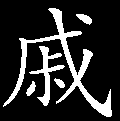
\includegraphics[width=3mm]{../Images/00005}  \kaishu 此回着重在宝琴,却出色写湘云。写湘云联句极敏捷聪慧,而宝琴之联句不少于湘云,可知出色写湘云,正所以出色写宝琴。出色写宝琴者,全为与宝玉提亲作引也。金针暗渡,不可不知。}

话说薛宝钗道:``到底分个次序,让我写出来。''说着,便令众人拈阄为序。起首恰是李氏。{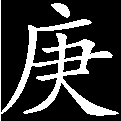
\includegraphics[width=3mm]{../Images/00004}  \kaishu 一定要按次序,恰又不按次序,似脱落处而不脱落,文章歧路如此。}然后按次各各开出。凤姐儿说道:``既是这样说,我也说一句在上头。''众人都笑说道:``更妙了!''宝钗便将稻香老农之上补了一个``凤''字,李纨又将题目讲与他听。凤姐儿想了半日,笑道:``你们别笑话我。我只有一句粗话,下剩的我就不知道了。''众人都笑道:``越是粗话越好,你说了只管干正事去罢。''凤姐儿笑道:``我想下雪必刮北风。昨夜听见了一夜的北风,我有了一句,就是`一夜北风紧',可使得?''众人听了,都相视笑道:``这句虽粗,不见底下的,这正是会作诗的起法。不但好,而且留了多少地步与后人。就是这句为首,稻香老农快写上续下去。''凤姐和李婶平儿又吃了两杯酒,自去了。这里李纨便写了:

一夜北风紧,

自己联道:

开门雪尚飘。入泥怜洁白,

香菱道:

匝地惜琼瑶。有意荣枯草,

探春道:

无心饰萎苕。价高村酿熟,

李绮道:

年稔府粱饶。葭动灰飞管,

李纹道:

阳回斗转杓。寒山已失翠,

岫烟道:

冻浦不闻潮。易挂疏枝柳,

湘云道:

难堆破叶蕉。麝煤融宝鼎,

宝琴道:

绮袖笼金貂。光夺窗前镜,

黛玉道:

香粘壁上椒。斜风仍故故,

宝玉道:

清梦转聊聊。何处梅花笛?

宝钗道:

谁家碧玉箫?鳌愁坤轴陷,

李纨笑道:``我替你们看热酒去罢。''宝钗命宝琴续联,只见湘云站起来道:

龙斗阵云销。野岸回孤棹,

宝琴也站起道:

吟鞭指灞桥。赐裘怜抚戍,

湘云那里肯让人,且别人也不如他敏捷,都看他扬眉挺身的说道:

加絮念征徭。坳垤审夷险,

宝钗连声赞好,也便联道:

枝柯怕动摇。皑皑轻趁步,

黛玉忙联道:

剪剪舞随腰。煮芋成新赏,

一面说,一面推宝玉,命他联。宝玉正看宝钗、宝琴、黛玉三人共战湘云,十分有趣,那里还顾得联诗,今见黛玉推他,方联道:

撒盐是旧谣。苇蓑犹泊钓,

湘云笑道:``你快下去,你不中用,倒耽搁了我。''一面只听宝琴联道:

林斧不闻樵。伏象千峰凸,

湘云忙联道:

盘蛇一径遥。花缘经冷结,

宝钗与众人又忙赞好。探春又联道:

色岂畏霜凋。深院惊寒雀,

湘云正渴了,忙忙的吃茶,已被岫烟道:

空山泣老鸮。阶墀随上下,

湘云忙丢了茶杯,忙联道:

池水任浮漂。照耀临清晓,

黛玉联道:

缤纷入永宵。诚忘三尺冷,

湘云忙笑联道:

瑞释九重焦。僵卧谁相问,

宝琴也忙笑联道:

狂游客喜招。天机断缟带,

湘云又忙道:

海市失鲛绡。

林黛玉不容他出,接着便道:

寂寞对台榭,

湘云忙联道:

清贫怀箪瓢。

宝琴也不容情,也忙道:

烹茶冰渐沸,

湘云见这般,自为得趣,又是笑,又忙联道:

煮酒叶难烧。

黛玉也笑道:

没帚山僧扫,

宝琴也笑道:

埋琴稚子挑。

湘云笑的弯了腰,忙念了一句,众人问:``到底说的什么?''湘云喊道:

石楼闲睡鹤,

黛玉笑的握着胸口,高声嚷道:

锦罽暖亲猫。

宝琴也忙笑道:

月窟翻银浪,

湘云忙联道:

霞城隐赤标。

黛玉忙笑道:

沁梅香可嚼,

宝钗笑称好,也忙联道:

淋竹醉堪调。

宝琴也忙道:

或湿鸳鸯带,

湘云忙联道:

时凝翡翠翘。

黛玉又忙道:

无风仍脉脉,

宝琴又忙笑联道:

不雨亦潇潇。

湘云伏着已笑软了。众人看他三人对抢,也都不顾作诗,看着也只是笑。黛玉还推他往下联,又道:``你也有才尽之时。我听听还有什么舌根嚼了!''湘云只伏在宝钗怀里,笑个不住。宝钗推他起来道:``你有本事,把`二萧'的韵全用完了,我才伏你。''湘云起身笑道:``我也不是作诗,竟是抢命呢。''众人笑道:``倒是你说罢。''探春早已料定没有自己联的了,便早写出来,因说:``还没收住呢。''李纹听了,接过来便联了一句道:

欲志今朝乐,

李绮收了一句道:

凭诗祝舜尧。

李纨道:``够了,够了。虽没作完了韵,剩的字若生扭用了,倒不好了。''说着,大家来细细评论一回,独湘云的多,都笑道:``这都是那块鹿肉的功劳。''

李纨笑道:``逐句评去都还一气,只是宝玉又落了第了。''宝玉笑道:``我原不会联句,只好担待我罢。''李纨笑道:``也没有社社担待你的。又说韵险了,又整误了,又不会联句了,今日必罚你。我才看见栊翠庵的红梅有趣,我要折一枝来插瓶。可厌妙玉为人,我不理他。如今罚你去取一枝来。''众人都道这罚的又雅又有趣。宝玉也乐为,答应着就要走。湘云黛玉一齐说道:``外头冷得很,你且吃杯热酒再去。''湘云早执起壶来,黛玉递了一个大杯,满斟了一杯。湘云笑道:``你吃了我们的酒,你要取不来,加倍罚你。''宝玉忙吃一杯,冒雪而去。

李纨命人好好跟着,黛玉忙拦说:``不必,有了人反不得了。''李纨点头说:``是。''一面命丫鬟将一个美女耸肩瓶拿来,贮了水准备插梅,因又笑道:``回来该咏红梅了。''湘云忙道:``我先作一首。''宝钗忙道:``今日断乎不容你再作了。你都抢了去,别人都闲着,也没趣。回来还罚宝玉,他说不会联句,如今就叫他自己作去。''{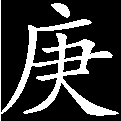
\includegraphics[width=3mm]{../Images/00004}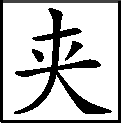
\includegraphics[width=3mm]{../Images/00012}\footnotesize \kaishu 想此刻宝玉已到庵中矣。}黛玉笑道:``这话很是。我还有个主意,方才联句不够,莫若拣着联的少的人作红梅。''宝钗笑道:``这话是极。方才邢李三位屈才,且又是客。琴儿和颦儿云儿三个人也抢了许多,我们一概都别作,只让他三个作才是。''李纨因说:``绮儿也不大会作,还是让琴妹妹作罢。''宝钗只得依允,{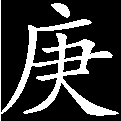
\includegraphics[width=3mm]{../Images/00004}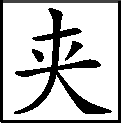
\includegraphics[width=3mm]{../Images/00012}\footnotesize \kaishu 想此刻二玉已会,不知肯见赐否?}又道:``就用`红梅花'三个字作韵,每人一首七律。邢大妹妹作`红'字,你们李大妹妹作`梅'字,琴儿作`花'字。''李纨道:``饶过宝玉去,我不服。''湘云忙道:``有个好题目命他作。''众人问何题目?湘云道:``命他就作`访妙玉乞红梅',岂不有趣?''众人听了,都说有趣。

一语未了,只见宝玉笑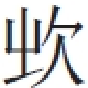
\includegraphics[width=4mm]{../images/00025}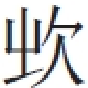
\includegraphics[width=4mm]{../images/00025}掮了一枝红梅进来。众丫鬟忙已接过,插入瓶内。众人都笑称谢。宝玉笑道:``你们如今赏罢,也不知费了我多少精神呢。''说着,探春早又递过一钟暖酒来,众丫鬟走上来接了蓑笠掸雪。各人房中丫鬟都添送衣服来,{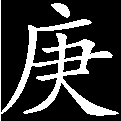
\includegraphics[width=3mm]{../Images/00004}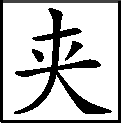
\includegraphics[width=3mm]{../Images/00012}\footnotesize \kaishu 冬日午后景况。}袭人也遣人送了半旧的狐腋褂来。李纨命人将那蒸的大芋头盛了一盘,又将朱橘、黄橙、橄榄等物盛了两盘,命人带与袭人去。湘云且告诉宝玉方才的诗题,又催宝玉快作。宝玉道:``姐姐妹妹们,让我自己用韵罢,别限韵了。''众人都说:``随你作去罢。''

一面说一面大家看梅花。原来这枝梅花只有二尺来高,旁有一横枝纵横而出,约有五六尺长,其间小枝分歧,或如蟠螭,或如僵蚓,或孤削如笔,或密聚如林,花吐胭脂,香欺兰蕙,{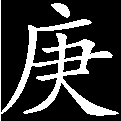
\includegraphics[width=3mm]{../Images/00004}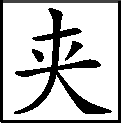
\includegraphics[width=3mm]{../Images/00012}\footnotesize \kaishu 一篇《红梅赋》。}各各称赏。谁知邢岫烟、李纹、薛宝琴三人都已吟成,各自写了出来。众人便依``红梅花''三字之序看去,写道是:

咏红梅花{得``红''字 邢岫烟}

桃未芳菲杏未红,冲寒先已笑东风。

魂飞庾岭春难辨,霞隔罗浮梦未通。

绿萼添妆融宝炬,缟仙扶醉跨残虹。

看来岂是寻常色,浓淡由他冰雪中。

咏红梅花{得``梅''字 李纹}

白梅懒赋赋红梅,逞艳先迎醉眼开。

冻脸有痕皆是血,酸心无恨亦成灰。

误吞丹药移真骨,偷下瑶池脱旧胎。

江北江南春灿烂,寄言蜂蝶漫疑猜。

咏红梅花{得``花''字 薛宝琴}

疏是枝条艳是花,春妆儿女竞奢华。

闲庭曲槛无馀雪,流水空山有落霞。

幽梦冷随红袖笛,游仙香泛绛河槎。

前身定是瑶台种,无复相疑色相差。

众人看了,都笑称赞了一番,又指末一首说更好。宝玉见宝琴年纪最小,才又敏捷,深为奇异。黛玉湘云二人斟了一小杯酒,齐贺宝琴。宝钗笑道:``三首各有各好。你们两个天天捉弄厌了我,如今捉弄他来了。''李纨又问宝玉:``你可有了?''宝玉忙道:``我倒有了,才一看见那三首,又吓忘了,等我再想。''湘云听了,便拿了一支铜火箸击着手炉,笑道:``我击鼓了,若鼓绝不成,又要罚的。''宝玉笑道:``我已有了。''黛玉提起笔来,说道:``你念,我写。''湘云便击了一下笑道:``一鼓绝。''宝玉笑道:``有了,你写吧。''众人听他念道:

酒未开樽句未裁,

黛玉写了,摇头笑道:``起的平平。''湘云又道``快着!''宝玉笑道:

寻春问腊到蓬莱。

黛玉湘云都点头笑道:``有些意思了。''宝玉又道:

不求大士瓶中露,为乞嫦娥槛外梅。

黛玉写了,又摇头道:``凑巧而已。''湘云忙催二鼓,宝玉又笑道:

入世冷挑红雪去,离尘香割紫云来。

槎枒谁惜诗肩瘦,衣上犹沾佛院苔。

黛玉写毕,湘云大家才评论时,又见几个丫鬟跑进来道:``老太太来了。''

众人忙迎出来。大家又笑道:``怎么这等高兴!''说着,远远见贾母围了大斗篷,带着灰鼠暖兜,坐着小竹轿,打着青绸油伞,鸳鸯琥珀等五六个丫鬟,每人都是打着伞,拥轿而来。李纨等忙往上迎,贾母命人止住说:``只在那里就是了。''来至跟前,贾母笑道:``我瞒着你太太和凤丫头来了。大雪地下坐着这个无妨,没的叫他们来踩雪。''众人忙一面上前接斗篷,搀扶着,一面答应着。贾母来至室中,先笑道:``好俊梅花!你们也会乐,我来着了。''说着,李纨早命拿了一个大狼皮褥来铺在当中。贾母坐了,因笑道:``你们只管顽笑吃喝。我因为天短了,不敢睡中觉,抹了一回牌,想起你们来了,我也来凑个趣儿。''李纨早又捧过手炉来,探春另拿了一副杯箸来,亲自斟了暖酒,奉与贾母。贾母便饮了一口,问那个盘子里是什么东西。众人忙捧了过来,回说是糟鹌鹑。贾母道:``这倒罢了,撕一两点腿子来。''李纨忙答应了,要水洗手,亲自来撕。贾母又道:``你们仍旧坐下说笑我听。''又命李纨:``你也坐下,就如同我没来的一样才好,不然我就去了。''众人听了,方依次坐下,这李纨便挪到尽下边。贾母因问作何事了,众人便说作诗。贾母道:``有作诗的,不如作些灯谜,大家正月里好顽的。''众人答应了。说笑了一回,贾母便说:``这里潮湿,你们别久坐,仔细受了潮湿。''因说:``你四妹妹那里暖和,我们到那里瞧瞧他的画儿,赶年可有了。''众人笑道:``那里能年下就有了?只怕明年端阳有了。''贾母道:``这还了得!他竟比盖这园子还费工夫了。''

说着,仍坐了竹轿,大家围随,过了藕香榭,穿入一条夹道,东西两边皆有过街门,门楼上里外皆嵌着石头匾,如今进的是西门,向外的匾上凿着``穿云''二字,向里的凿着``度月''两字。来至当中,进了向南的正门,贾母下了轿,惜春已接了出来。从里边游廊过去,便是惜春卧房,门斗上有``暖香坞''三个字。{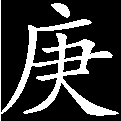
\includegraphics[width=3mm]{../Images/00004}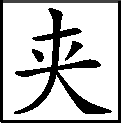
\includegraphics[width=3mm]{../Images/00012}\footnotesize \kaishu 看他又写出一处,从起至末一笔一部之文也有,千万笔成一部之文也有,一二笔成一部之文也有。如``试才''一回起若都说完,以后则索然无味,故留此几处以为后文之点染也。此方活泼不板,眼目屡新。}早有几个人打起猩红毡帘,已觉温香拂脸。{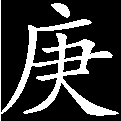
\includegraphics[width=3mm]{../Images/00004}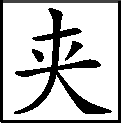
\includegraphics[width=3mm]{../Images/00012}\footnotesize \kaishu 各处皆如此,非独因``暖香''二字方有此景。戏注于此,以博一笑耳。}大家进入房中,贾母并不归坐,只问画在那里。惜春因笑回:``天气寒冷了,胶性皆凝涩不润,画了恐不好看,故此收起来。''贾母笑道:``我年下就要的。你别托懒儿,快拿出来给我快画。''一语未了,忽见凤姐儿披着紫羯绒褂,笑嘻嘻的来了,口内说道:``老祖宗今儿也不告诉人,私自就来了,要我好找。''贾母见他来了,心中自是喜悦,便道:``我怕你们冷着了,所以不许人告诉你们去。你真是个鬼灵精儿,到底找了我来。以理,孝敬也不在这上头。''凤姐儿笑道:``我那里是孝敬的心找了来?我因为到了老祖宗那里,鸦没雀静的,{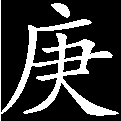
\includegraphics[width=3mm]{../Images/00004}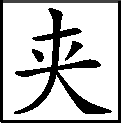
\includegraphics[width=3mm]{../Images/00012}\footnotesize \kaishu 这四个字俗语中常闻,但不能落纸笔耳。便欲写时,究竟不知系何四字,今如此写来,真是不可移易。}问小丫头子们,他又不肯说,叫我找到园里来。我正疑惑,忽然来了两三个姑子,我心里才明白。我想姑子必是来送年疏,或要年例香例银子,老祖宗年下的事也多,一定是躲债来了。我赶忙问了那姑子,果然不错。我连忙把年例给了他们去了。如今来回老祖宗,债主已去,不用躲着了。已预备下希嫩的野鸡,请用晚饭去,再迟一回就老了。''他一行说,众人一行笑。

凤姐儿也不等贾母说话,便命人抬过轿子来。贾母笑着,搀了凤姐的手,仍旧上轿,带着众人,说笑出了夹道东门。一看四面粉妆银砌,忽见宝琴披着凫靥裘站在山坡上遥等,身后一个丫鬟抱着一瓶红梅。众人都笑道:``少了两个人,他却在这里等着,也弄梅花去了。''贾母喜的忙笑道:``你们瞧,这山坡上配上他的这个人品,又是这件衣裳,后头又是这梅花,像个什么?''众人都笑道:``就像老太太屋里挂的仇十洲画的《双艳图》。''贾母摇头笑道:``那画的那里有这件衣裳?人也不能这样好!''一语未了,只见宝琴背后转出一个披大红猩毡的人来。贾母道:``那又是那个女孩儿?''众人笑道:``我们都在这里,那是宝玉。''贾母笑道:``我的眼越发花了。''说话之间,来至跟前,可不是宝玉和宝琴。宝玉笑向宝钗黛玉等道:``我才又到了栊翠庵。妙玉每人送你们一枝梅花,我已经打发人送去了。''众人都笑说:``多谢你费心。''

说话之间,已出了园门,来至贾母房中。吃毕饭大家又说笑了一回。忽见薛姨妈也来了,说:``好大雪,一日也没过来望候老太太。今日老太太倒不高兴?正该赏雪才是。''贾母笑道:``何曾不高兴!我找了他们姊妹们去顽了一会子。''薛姨妈笑道:``昨日晚上,我原想着今日要和我们姨太太借一日园子,摆两桌粗酒,请老太太赏雪的,又见老太太安息的早。我闻得女儿说,老太太心下不大爽,因此今日也没敢惊动。早知如此,我正该请。''贾母笑道:``这才是十月里头场雪,往后下雪的日子多呢,再破费不迟。''薛姨妈笑道:``果然如此,算我的孝心虔了。''凤姐儿笑道:``姨妈仔细忘了,如今先秤五十两银子来,交给我收着,一下雪,我就预备下酒,姨妈也不用操心,也不得忘了。''贾母笑道:``既这么说,姨太太给他五十两银子收着,我和他每人分二十五两,到下雪的日子,我装心里不快,混过去了,姨太太更不用操心,我和凤丫头倒得了实惠。''凤姐将手一拍,笑道:``妙极了,这和我的主意一样。''众人都笑了。贾母笑道:``呸!没脸的,就顺着竿子爬上来了!你不说姨太太是客,在咱们家受屈,我们该请姨太太才是,那里有破费姨太太的理!不这样说呢,还有脸先要五十两银子,真不害臊!''凤姐儿笑道:``我们老祖宗最是有眼色的,试一试,姨妈若松呢,拿出五十两来,就和我分。这会子估量着不中用了,翻过来拿我做法子,说出这些大方话来。如今我也不和姨妈要银子,竟替姨妈出银子治了酒,请老祖宗吃了,我另外再封五十两银子孝敬老祖宗,算是罚我个包揽闲事。这可好不好?''话未说完,众人已笑倒在炕上。

贾母因又说及宝琴雪下折梅比画儿上还好,因又细问他的年庚八字并家内景况。薛姨妈度其意思,大约是要与宝玉求配。薛姨妈心中固也遂意,只是已许过梅家了,因贾母尚未明说,自己也不好拟定,遂半吐半露告诉贾母道:``可惜这孩子没福,前年他父亲就没了。他从小儿见的世面倒多,跟他父母四山五岳都走遍了。他父亲是好乐的,各处因有买卖,带着家眷,这一省逛一年,明年又往那一省逛半年,所以天下十停走了有五六停了。那年在这里,把他许了梅翰林的儿子,偏第二年他父亲就辞世了,他母亲又是痰症。''凤姐也不等说完,便嗐声跺脚的说:``偏不巧,我正要作个媒呢,又已经许了人家。''贾母笑道:``你要给谁说媒?''凤姐儿说道:``老祖宗别管,我心里看准了他们两个是一对。如今已许了人,说也无益,不如不说罢了。''贾母也知凤姐儿之意,听见已有了人家,也就不提了。大家又闲话了一会方散。一宿无话。

次日雪晴。饭后,贾母又亲嘱惜春:``不管冷暖,你只画去,赶到年下,十分不能便罢了。第一要紧把昨日琴儿和丫头梅花,照模照样,一笔别错,快快添上。''惜春听了虽是为难,只得应了。一时众人都来看他如何画,惜春只是出神。李纨因笑向众人道:``让他自己想去,咱们且说话儿。昨儿老太太只叫作灯谜,回家和绮儿纹儿睡不着,我就编了两个`四书'的。他两个每人也编了两个。''众人听了,都笑道:``这倒该作的。先说了,我们猜猜。''李纨笑道:``\,`观音未有世家传',打《四书》一句。''湘云接着就说``在止于至善。''宝钗笑道:``你也想一想`世家传'三个字的意思再猜。''李纨笑道:``再想。''黛玉笑道:``哦,是了。是`虽善无征'。''众人都笑道:``这句是了。''李纨又道:``一池青草草何名。''湘云忙道:``这一定是`蒲芦也'。再不是不成?''李纨笑道:``这难为你猜。纹儿的是`水向石边流出冷',打一古人名。''探春笑问道:``可是山涛?''李纹笑道:``是。''李纨又道:``绮儿的是个`萤'字,打一个字。''众人猜了半日,宝琴笑道:``这个意思却深,不知可是花草的`花'字?''李绮笑道:``恰是了。''众人道:``萤与花何干?''黛玉笑道:``妙得很!萤可不是草化的?''众人会意,都笑了说;``好!''宝钗道:``这些虽好,不合老太太的意思,不如作些浅近的物儿,大家雅俗共赏才好。''众人都道:``也要作些浅近的俗物才是。''湘云笑道:``我编了一支《点绛唇》,恰是俗物,你们猜猜。''说着便念道:

溪壑分离,红尘游戏,真何趣?名利犹虚,后事终难继。

众人不解,想了半日,也有猜是和尚的,也有猜是道士的,也有猜是偶戏人的。宝玉笑了半日,道:``都不是,我猜着了,一定是耍的猴儿。''湘云笑道:``正是这个了。''众人道:``前头都好,末后一句怎么解?''湘云道:``那一个耍的猴子不是剁了尾巴去的?''众人听了,都笑起来,说:``偏他编个谜儿也是刁钻古怪的。''李纨道:``昨日姨妈说,琴妹妹见的世面多,走的道路也多,你正该编谜儿,正用着了。你的诗且又好,何不编几个我们猜一猜?''宝琴听了,点头含笑,自去寻思。宝钗也有了一个,念道:

镂檀锲梓一层层,岂系良工堆砌成?

虽是半天风雨过,何曾闻得梵铃声!

打一物。

众人猜时,宝玉也有了一个,念道:

天上人间两渺茫,琅玕节过谨堤防。

鸾音鹤信须凝睇,好把唏嘘答上苍。

黛玉也有了一个,念道是:

騄駬何劳缚紫绳?驰城逐堑势狰狞。

主人指示风雷动,鳌背三山独立名。

探春也有了一个,方欲念时,宝琴走过来笑道:``我从小儿所走的地方的古迹不少,我今拣了十个地方的古迹,作了十首怀古的诗。诗虽粗鄙,却怀往事,又暗隐俗物十件,姐姐们请猜一猜。''众人听了,都说:``这倒巧,何不写出来大家一看?''要知端的------

{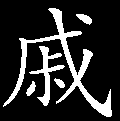
\includegraphics[width=3mm]{../Images/00005}  \kaishu 总评:诗词之俏丽、灯谜之隐秀不待言,须看他极整齐、极参差,愈忙迫愈安闲,一波一折路转峰回,一落一起山断云连,各人局度、各人情性都现。至李纨主坛,而起句却在凤姐,李纨主坛,而结句却在最少之李绮,另是一样弄奇。}

{最爱他中幅惜春作画一段,似与本文无涉,而前后文之景色人物,莫不筋动脉摇,而前后文之起伏照应,莫不穿插映带。文字之奇,难以言状。}
